\providecommand{\main}{../../..}
\documentclass[\main/dresen_thesis.tex]{subfiles}

\begin{document}
  \subsection{D33}\label{ch:lss:d33}
    \begin{figure}[ht]
      \centering
      \includegraphics[width=0.7\textwidth]{appendix_instruments_d33}
      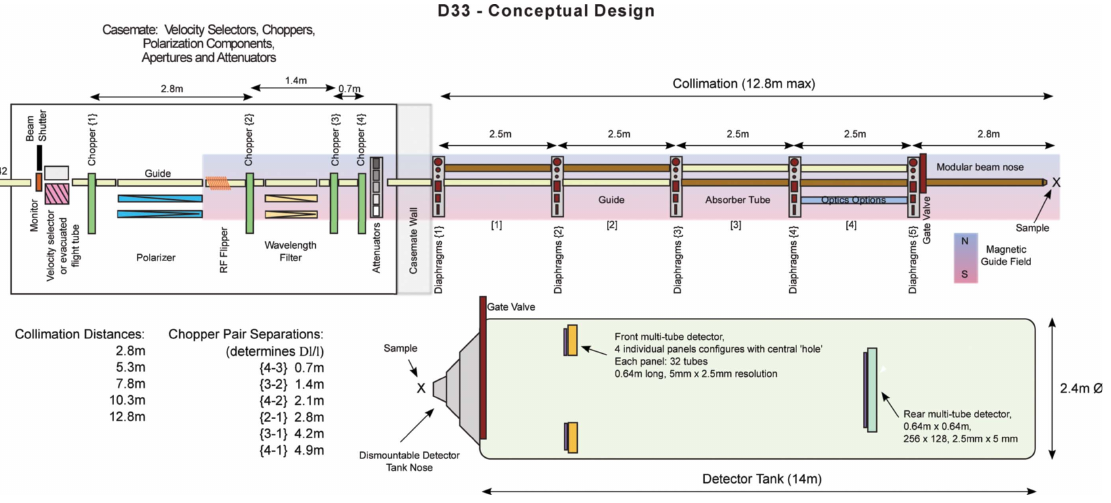
\includegraphics[width=0.7\textwidth]{appendix_instruments_d33Setup}
      \caption{\label{fig:lss:d33}D33 instrument at Institut Laue-Langevin used for (grazing incidence) small angle scattering with (polarized) neutrons (schematics reproduced from \cite{Dewhurst_2015_Thesm}).}
    \end{figure}
    The D33 instrument \cite{Dewhurst_2015_Thesm} at the Institut Laue-Langevin is used to measure small-angle scattering of polarised neutrons for dispersions, as well as for samples on a substrate under grazing-incidence.
    Similar to D17 \ref{ch:lss:d17} it can be used in monochromatic and TOF mode, where in this thesis the monochromatic mode is chosen for all measurements.
    The Astrium EADS velocity selector can be used to select a wavelength in the range of $4.5 \ldots 40 \unit{\angstrom}$ with a energy resolution of $10 \unit{\%}$ (FWHM).
    It has an adjustable collimation-to-sample and sample-to-detector distance, which can be chosen incrementally in the range $L_\mathrm{CSD} \eq 2.8 \ldots 12.8 \unit{m}$ and $L_\mathrm{SSD} \eq 1.2 \ldots 12.8 \unit{m}$ respectively.
    The collimation is chosen analogue to D22 by the aid of four $2.5 \unit{m}$ changer sections, which can either be a neutron guide of an empty flight path with an absorbing boron carbide lined tube and antiparasitic baffles.
    The angular divergence can thereby be defined between $0.01^\circ \ldots 0.31^\circ$, depending on the chosen lengths and apertures.
    The detector has a pixel size of $5 \times 5 \unit{mm^2}$ and $128 \times 128$ pixels.

    The neutron polarisation is obtained by the insertion of a \ch{Fe}/\ch{Si} multilayer mirror close to the velocity selector between the chopper system of D33 with a single-blade mirror for long wavelengths and a V-shaped mirror for short wavelengths.
    The RF flipper is installed close to the polarizer and can be turned on and off during SANSPOL measurements to set the spin direction of the incoming neutrons.
    The polarization efficiency of this mirror system is in the order of $>95 \unit{\%}$, where the flipping efficiency is $>99 \unit{\%}$.

    The data reduction including the correction for polarization efficiency, as well as detector sensitivity can be performed using the Matlab script GRASP \cite{Dewhurst_2003_Grasp}.
\end{document}